\chapter{Background}
The methods developed in this thesis build on foundational concepts from \gls{rl}, \gls{marl}, and quadrotors. We begin with an overview of model free, on policy policy optimization, introducing Markov decision processes, policy gradients, and \gls{ppo}. These ideas are then extended to cooperative multi agent tasks, comparing centralized critics with fully decentralized critics. Next, we present the mathematical model of a quadrotor \gls{uav}, including coordinate frames, state representation, sensor fusion, continuous time dynamics, and common action space formulations ranging from velocity commands to direct thrust control. Finally, we describe how the quadrotor state is augmented for cable suspended payloads—first via a simple pendulum model and then through multi link or tendon based approximations—and explain how these formulations generalize to cooperative transport by multiple \glspl{uav}. These foundations are essential for the development a deep \gls{rl} framework for decentralized multi-\gls{uav} cable-suspended payload transport.

\section{Fundamentals of Reinforcement Learning}
The term \gls{rl} is used for a wide range of algorithms and methods that learn to make decisions by interacting with an environment. The following will give a brief overview of the most important concepts and terms in \gls{rl}. In particular, this work focuses on model-free, on-policy, policy-optimization algorithms, where the policy used to collect data is the same one being updated. For a thorough treatment of the fundamentals see \cite{SuttonBarto2018}.
\subsection{Markov Decision Processes}
\begin{figure}
\centering
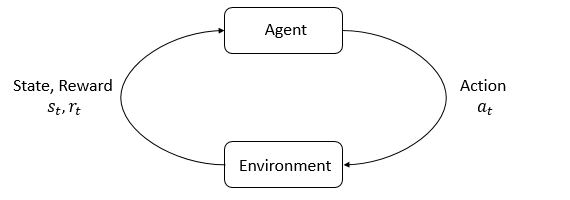
\includegraphics[width=0.8\textwidth]{images/rl_diagram.png}
\caption{TODO   Reinforcement learning framework. The agent interacts with the environment by taking actions and receiving rewards, while the environment transitions to new states based on the agent's actions.}
\label{fig:rl_diagram}
\end{figure}

\gls{rl} is a framework in which an agent learns to make decisions by interacting with its environment.  This interaction is commonly modeled as a \gls{mdp}, defined by the tuple
\[
(\mathcal{S}, \mathcal{A}, P, r, \gamma),
\]
where \(\mathcal{S}\) is the set of all possible states; \(\mathcal{A}\) is the set of all possible actions; \(P(s'\!\mid\!s,a)\) is the probability of transitioning to \(s'\) from \(s\) when taking \(a\); \(r(s,a)\) is the immediate reward for taking action \(a\) in state \(s\); and \(\gamma\in[0,1)\) is the discount factor, which down-weights future rewards.

At each time step \(t\), the agent interacts with the environment as also shown in Figure~\ref{fig:rl_diagram}. The agent observes \(s_t\); samples \(a_t\sim\pi_\theta(\cdot\mid s_t)\); receives \(r_t = r(s_t,a_t)\); and transitions to \(s_{t+1}\sim P(\cdot\mid s_t,a_t)\). In practice the agent often does not have access to the full state \(s_t\) but only to a partial observation \(o_t\).  We will use the notation interchangeably, i.e.\ \(o_t\) or \(s_t\) depending on the context, unless otherwise specified.
\subsection{Policies}
As already mentioned, the agent's behavior is defined by a policy \(\pi_\theta\), which can be either deterministic or stochastic:
 
    \[
      a_t = \pi_{\theta}(s_t),
    \]
    where \(\pi_{\theta}\) is a deterministic function (e.g., a neural network) mapping state \(s_t\) to action \(a_t\).

    \[
      a_t \sim \pi_{\theta}(\,\cdot\mid s_t),
    \]
    where \(\pi_{\theta}(a\mid s_t)\) is the probability of taking action \(a\) in state \(s_t\).
We parameterize \(\pi_{\theta}\) with \(\theta\) and optimize it to maximize the expected return. Typically, the policy is represented by a neural network taking \(s_t\) as input.

\subsection{Reward and Return}
The agent's goal is to maximize the expected return, which is the total discounted reward over time. 
The reward function \(r_t(s_t,a_t)\) provides immediate feedback to the agent and usually depends on the current state \(s\), action taken by the policy \(a\) and the next state \(s'\). The return \(R_t\) at time step \(t\) is defined as the sum of discounted rewards:
\[
R_t = \sum_{k=0}^{\infty} \gamma^k r_{t+k},
\]
where \(\gamma\) is the discount factor that determines the importance of future rewards. The expected return \(J(\pi)\) is defined as the expected value of the return:

\[
J(\pi) = \mathbb{E}\Bigl[\sum_{t=0}^\infty \gamma^t\,R_t\Bigr].
\]

At every time step \(t\), the agent observes the current state \(s_t\), selects an action \(a_t\) according to a policy \(\pi(a_t\mid s_t)\), receives an immediate reward \(r(s_t,a_t)\), and transitions to the next state \(s_{t+1}\) based on the dynamics \(P\). The goal is to find the optimal policy \(\pi^*\) that maximizes the expected total discounted reward if the agent acts according to it. This formulation can be explicitly stated as the following constrained optimization problem:
\begin{equation}\label{eq:RL_opt}
\begin{aligned}
\text{Find} \quad & \pi^* = \arg\max_{\pi} \mathbb{E}\left[J(\pi)\right] \\
\text{subject to} \quad & s_0 \sim \rho_0, \\
& a_t \sim \pi(\cdot \mid s_t), \quad \forall\ t \in T \\
& s_{t+1} \sim P(\cdot \mid s_t, a_t)
\end{aligned}
\end{equation}

\subsection{Value and Action-Value Functions}

Given a fixed policy \(\pi_\theta\), we define two key quantities that measure expected return:

\[
V^\pi(s) = \mathbb{E}\Bigl[\sum_{t=0}^{\infty} \gamma^t\,r_t \;\Big|\; s_0 = s\Bigr], 
\qquad
Q^\pi(s,a) = \mathbb{E}\Bigl[\sum_{t=0}^{\infty} \gamma^t\,r_t \;\Big|\; s_0 = s,\; a_0 = a\Bigr].
\]

Here, \(V^\pi(s)\) is the expected discounted return starting from state \(s\) under \(\pi_\theta\), and \(Q^\pi(s,a)\) is the expected discounted return starting from \(s\), taking action \(a\), then following \(\pi_\theta\). 

The Bellman equations decompose each function into reward received until the current state and the discounted value of the next state and action:

\begin{align}
\label{eq:BellmanV}
V^\pi(s)
&= \mathbb{E}_{a\sim\pi(\cdot\mid s)}\bigl[r(s,a)\bigr]
  + \gamma\,\mathbb{E}_{\substack{a\sim\pi(\cdot\mid s)\\s'\sim P(\cdot\mid s,a)}}\bigl[V^\pi(s')\bigr],\\[4pt]
\label{eq:BellmanQ}
Q^\pi(s,a)
&= \mathbb{E}_{s'\sim P(\cdot\mid s,a)}\bigl[r(s,a)\bigr]
  + \gamma\,\mathbb{E}_{\substack{s'\sim P(\cdot\mid s,a)\\a'\sim\pi(\cdot\mid s')}}\bigl[Q^\pi(s',a')\bigr].
\end{align}

The Bellman equations can be combined to give us the advantage function \(A^\pi\), which quantifies the relative value of taking action \(a\) in state \(s\) compared to the average value of the state:
\begin{align}
\label{eq:advantage}
A^\pi(s,a)
&= Q^\pi(s,a) - V^\pi(s)
\end{align}

\subsection{On-Policy Policy-Gradient Loop}  
On-policy methods repeatedly collect fresh data under \(\pi_\theta\) to perform stochastic gradient ascent on \(J(\theta)\) to ultimately improve the policy towards \(\pi^*\). The gradient can be derived from the advantage function \(A^\pi\) as
\begin{align}
\label{eq:policy_gradient}
\nabla_\theta J(\theta)
&= \mathbb{E}\Bigl[\sum_{t=0}^\infty \gamma^t\,\nabla_\theta \log \pi_\theta(a_t\mid s_t)\,A_t\Bigr],
\end{align}
In practice, there are different approaches to approximate the policy gradient \(\nabla_{\theta}J(\theta)\). In the next section, we will focus on the \gls{ppo} algorithm, which is a popular on-policy method, using a surrogate objective function to optimize the policy.

\subsection{PPO}
\gls{ppo} was introduced by Schulman et al. in \cite{schulman2017proximal}. \gls{ppo} is a family of policy gradient methods that strives for simplicity, efficiency, and robustness. Its central idea is to iteratively improve a stochastic policy by alternating between sampling data from the environment and performing several epochs of first-order optimization on a surrogate objective function. It is an on-policy algorithm.

In \gls{ppo}, actions are sampled from a parameterized probability distribution. For continuous control tasks, the actor typically outputs the parameters of a Gaussian distribution (usually the mean and standard deviation), and actions are sampled as
\[
a_t \sim \mathcal{N}\big(\mu_\theta(s_t),\, \sigma_\theta(s_t)\big).
\]
This stochastic sampling is crucial as it enables the agent to explore a continuous range of actions, thereby promoting both exploration and robustness in learning.

\gls{ppo} builds on the actor-critic framework, where two components are optimized simultaneously. The actor represents the policy \(\pi_\theta\), which selects actions, while the critic estimates a value function \(V_\theta(s)\) that evaluates the quality of states under the current policy. The critic is used to compute an advantage function that quantifies the relative benefit of taking a specific action in a given state. A commonly used method for estimating advantages is \gls{gae}, which effectively reduces variance while introducing a manageable bias that aids learning stability. \gls{gae} computes the advantage as
\[
\hat{A}_t = \sum_{l=0}^{\infty} (\gamma \lambda)^l \delta_{t+l},
\]
with the temporal difference error defined as
\[
\delta_t = r_t + \gamma V_\theta(s_{t+1}) - V_\theta(s_t).
\]
Here, \(r_t\) is the reward received at time \(t\), \(V_\theta(s_t)\) is the estimated value of state \(s_t\) under the current policy, \(\gamma \in [0,1]\) is the discount factor that weighs future rewards, and \(\lambda \in [0,1]\) is a parameter that adjusts the trade-off between bias and variance in the advantage estimates.

A key contribution of \gls{ppo} is the use of a clipped surrogate objective designed to restrict the size of policy updates. Let
\[
r_t(\theta) = \frac{\pi_\theta(a_t \mid s_t)}{\pi_{\theta_{\text{old}}}(a_t \mid s_t)}
\]
denote the probability ratio between the new and the old policies. The clipped surrogate objective is then defined as:
\[
L^{CLIP}(\theta) = \mathbb{E}_t\!\left[\min\!\left(r_t(\theta)\hat{A}_t,\;\text{clip}\left(r_t(\theta),\,1-\epsilon,\,1+\epsilon\right)\hat{A}_t\right)\right],
\]
where \(\hat{A}_t\) is an estimator of the advantage function and \(\epsilon\) is a hyperparameter defining the clipping range. This objective penalizes overly large deviations from the previous policy, ensuring that updates remain conservative while still allowing for meaningful improvements.

In practice, \gls{ppo} combines the policy surrogate loss with additional terms, such as a value function loss and an entropy bonus, yielding a composite objective:
\[
L(\theta) = \mathbb{E}_t \left[ L^{CLIP}_t(\theta) - c_1\, \left(V_\theta(s_t) - V_t^{\text{target}}\right)^2 + c_2\, S\big[\pi_\theta\big](s_t) \right],
\]
where \(c_1\) and \(c_2\) are coefficients that weight the contributions of the value function error and the entropy bonus \(S\big[\pi_\theta\big](s_t)\), respectively. This final objective is optimized using stochastic gradient ascent over multiple epochs on the same batch of on-policy samples.

The overall procedure of \gls{ppo} in an actor-critic setting is summarized in Algorithm~\ref{alg:ppo}. In the algorithm, \(\theta\) denotes the current policy parameters, \(\theta_{\text{old}}\) are the parameters used for generating the on-policy data, \(N\) is the number of parallel actors, \(T\) is the number of timesteps per actor rollout (with \(NT\) total timesteps per batch), \(K\) is the number of epochs over the data, and \(M \le NT\) is the minibatch size.


\begin{algorithm}[H]
\caption{\gls{ppo}, Actor-Critic Style}
\label{alg:ppo}
\begin{algorithmic}[1]
\For{iteration = 1, 2, \dots}
    \For{actor = 1, 2, \dots, N}
        \State Run policy \(\pi_{\theta_{\text{old}}}\) in the environment for \(T\) timesteps.
        \State Compute advantage estimates \(\hat{A}_1, \dots, \hat{A}_T\).
    \EndFor
    \State Optimize the surrogate loss \(L(\theta)\) with respect to \(\theta\) using \(K\) epochs and minibatch size \(M \le NT\).
    \State Update \(\theta_{\text{old}} \leftarrow \theta\).
\EndFor
\end{algorithmic}
\end{algorithm}

Overall, \gls{ppo} strikes a favorable balance between simplicity and performance, making it one of the most widely adopted on-policy algorithms in modern reinforcement learning applications. The following sections will discuss the multi-agent extensions of \gls{ppo} that are used in this work.
\section{Multi-Agent Reinforcement Learning}

This section provides an overview of the theoretical background of \gls{marl} as applied in this work. Our work evaluates both centralized and decentralized training paradigms. In particular, we employ Proximal Policy Optimization (PPO) for centralized training, while also exploring decentralized approaches using Independent PPO (IPPO) and Multi-Agent PPO (MAPPO), which are detailed in subsequent sections.


\section{Multi-Agent Markov Decision Process}
A cooperative multi-agent reinforcement learning problem can be formalized as a \gls{dec-pomdp}\cite{oliehoek_concise_2016}, defined by the tuple
\[
  \bigl(\mathcal{N},\,\mathcal{S},\,\{\mathcal{A}^i\}_{i=1}^N,\,P,\,r,\,\{\Omega^i\}_{i=1}^N,\,O,\,\gamma\bigr)
\]
where $\mathcal{N}=\{1,\dots,N\}$ is the set of agents; $\mathcal{S}$ is the set of global states (with $s_0\sim\rho(s)$ denoting the initial state distribution); $\mathcal{A}^i$ is the action space of agent $i$, and the joint action space is $\mathcal{A} = \prod_{i=1}^N \mathcal{A}^i$; $P(s' \mid s, a)$ is the transition kernel, where $a=(a^1,\dots,a^N)\in\mathcal{A}$; $r(s,a)\in\mathbb{R}$ is the common team reward received by all agents; $\Omega^i$ is the observation space of agent $i$, and $O(o^1,\dots,o^N\mid s)$ is the joint observation function; and $\gamma\in[0,1)$ is the discount factor.
At each time step $t$, each agent $i$ receives a private observation $o^i_t \in \Omega^i$ sampled from $O(\cdot\mid s_t)$ and selects an action 
$a^i_t \sim \pi^i\bigl(a^i \mid \tau^i_t\bigr)$
conditioned on its action-observation history $\tau^i_t$. The joint policy 
$\pi(a\mid \tau) \;=\; \prod_{i=1}^N \pi^i\bigl(a^i\mid \tau^i\bigr)$
induces an expected discounted return
\[
  J(\pi) \;=\; \mathbb{E}\Bigl[\sum_{t=0}^\infty \gamma^t\,r(s_t, a_t)\Bigr]\,. 
\]

\section{\gls{ppo} in Multi-Agent Settings}
There is two main approaches to applying \gls{ppo} in multi-agent settings: \gls{ippo} and \gls{mappo}. Both approaches extend the single-agent \gls{ppo} algorithm to handle multiple agents, but they differ in how they address the challenges of non-stationarity and credit assignment in multi-agent environments. Their main difference is is wether the critics are centralized or decentralized. In \gls{ippo}, each agent has its own critic, while in \gls{mappo}, a shared critic is used across all agents. This section will provide a brief overview of both approaches.

\subsection{\gls{ippo}}
\gls{ippo} \cite{witt_is_2020} extends the single agent \gls{ppo} (clipped surrogate objective, GAE, value-loss and entropy bonus) for each agent in isolation, treating the other agents as part of the non-stationary environment.  Concretely, for each agent \(i\) we optimize
\[
  L_i(\theta_i) \;=\; 
  \mathbb{E}_t \Bigl[\,L^{\mathrm{CLIP}}_i(\theta_i) \;-\; c_1\,\bigl(V_{\phi_i}(o^i_t)-V^{\text{target},\,i}_t\bigr)^2
    \;+\; c_2\,S\bigl[\pi_{\theta_i}\bigr](o^i_t)\Bigr],
\]
where
\[
  L^{\mathrm{CLIP}}_i(\theta_i)
  = \mathbb{E}_t\!\Bigl[\min\bigl(r^i_t(\theta_i)\,\hat A^i_t,\;\mathrm{clip}(r^i_t(\theta_i),1-\epsilon,1+\epsilon)\,\hat A^i_t\bigr)\Bigr],
\]
\(r^i_t(\theta_i)\!=\!\frac{\pi_{\theta_i}(a^i_t\mid o^i_t)}{\pi_{\theta_i}^{\mathrm{old}}(a^i_t\mid o^i_t)}\), and \(\hat A^i_t\) is computed with \gls{gae} using the local critic \(V_{\phi_i}\).  Each agent collects on-policy rollouts of its own interaction trace \(\{(o^i_t,a^i_t,r_t)\}\) and applies \(K\) epochs of minibatch SGD exactly as in single agent \gls{ppo}.  While this simplicity enables straightforward scaling to many agents, it does not explicitly address the non stationarity introduced by concurrent learning: all stability and performance gains must emerge implicitly from \gls{ppo} conservative updates and entropy regularization.

\subsection{\gls{mappo}}
\gls{mappo} \cite{yu_surprising_2022} retains the \gls{ppo} surrogate and mixed objective but moves to a \gls{ctde} paradigm.  A single policy network \(\pi_\theta(a^i\mid o^i)\) with shared parameters \(\theta\) is used by all agents at execution, while training leverages a centralized critic \(V_\phi(s)\) receiving full state (or joint observations).  The joint optimization target becomes
\[
  L(\theta,\phi) = \mathbb{E}_t\Bigl[\,L^{\mathrm{CLIP}}(\theta)
   \;-\; c_1\bigl(V_\phi(s_t)-V^{\text{target}}_t\bigr)^2
   \;+\; c_2\sum_{i=1}^N S\bigl[\pi_\theta(\cdot\mid o^i_t)\bigr]\Bigr],
\]
where
\[
  L^{\mathrm{CLIP}}(\theta)
  = \mathbb{E}_t\!\Bigl[\min\bigl(r_t(\theta)\,\hat A_t,\;\mathrm{clip}(r_t(\theta),1-\epsilon,1+\epsilon)\,\hat A_t\bigr)\Bigr],
\]
with the joint ratio \(r_t(\theta)=\prod_i \frac{\pi_\theta(a^i_t\mid o^i_t)}{\pi_{\theta_{\text{old}}}(a^i_t\mid o^i_t)}\) or approximated per-agent, and \(\hat A_t\) estimated via \gls{gae} using the centralized value \(V_\phi\).  By conditioning the critic on the true global state, \gls{mappo} yields lower-variance advantage estimates and more accurate credit assignment, yet at test time each agent executes only on its local observation \(o^i\), preserving decentralization.  Shared policy parameters encourage coordination and parameter efficient scaling, while the \gls{ctde} split ensures stability through centralized learning.


\section{Quadrotor}
\label{sec:quadrotor_control}

\begin{figure}[t]
  \centering
  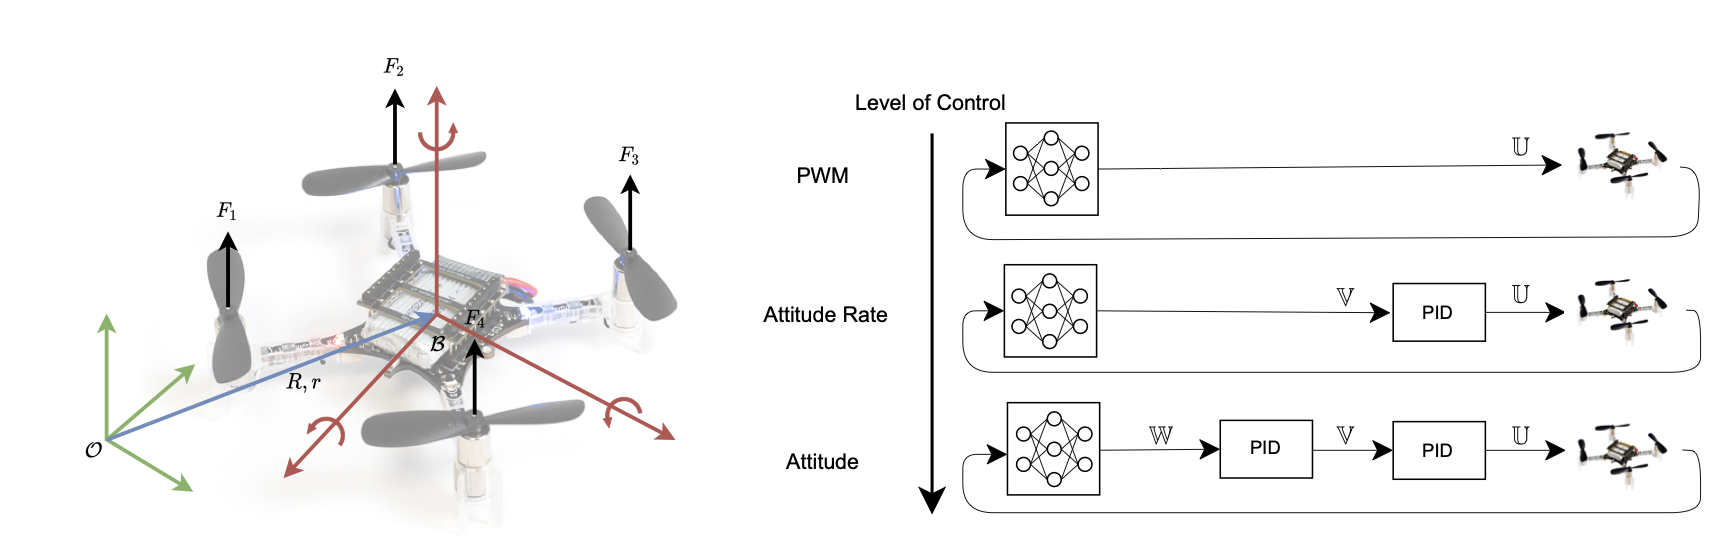
\includegraphics[width=0.8\textwidth]{quadrotor_dynamics.png}
  \caption{Diagram of the quadrotor showing the inertial frame \(\mathcal{I}\) and body frame \(\mathcal{B}\), as well as propeller numbering (1–4).}
  \label{fig:quadrotor_frames}
\end{figure}

Quadrotors are a class of rotorcraft \gls{uav} equipped with four fixed-pitch propellers. Each propeller generates thrust and a reactive torque, enabling attitude and position control. Quadrotors are widely used in applications such as aerial surveillance, package delivery, and search-and-rescue due to their mechanical simplicity and agility. In this chapter, we introduce the coordinate frames, state representation, onboard sensors, and fundamental dynamics and control action parameterizations for a quadrotor platform.

\subsection{Coordinate Frames and State Representation}
\label{sec:quadrotor_state}

We define two reference frames: the inertial (world) frame \(\mathcal{I}\) and the body-fixed frame \(\mathcal{B}\). The origin of \(\mathcal{B}\) is located at the quadrotor's center of mass, with its \(x\)-axis pointing forward, \(y\)-axis to the right, and \(z\)-axis upward (see Figure~\ref{fig:quadrotor_frames}). Let \(\mathbf{p}\in \mathbb{R}^{3}\) denote the position of the center of mass expressed in \(\mathcal{I}\), and let \(\mathbf{v} = \dot{\mathbf{p}}\in \mathbb{R}^{3}\) be the linear velocity in \(\mathcal{I}\). The attitude of the quadrotor is represented by a rotation matrix \(\mathbf{R} \in \mathrm{SO}(3)\) that maps vectors from \(\mathcal{B}\) to \(\mathcal{I}\). The angular velocity of the body, expressed in \(\mathcal{B}\), is denoted \(\boldsymbol{\omega} = [\omega_{x},\,\omega_{y},\,\omega_{z}]^{\mathsf{T}}\in \mathbb{R}^{3}\). We collect these variables into the state vector
\[
x = \bigl(\mathbf{p},\,\mathbf{v},\,\mathbf{R},\,\boldsymbol{\omega}\bigr)\,.
\]

\subsection{Sensors and State Estimation}
\label{sec:quadrotor_estimation}

The quadrotor's onboard state estimator fuses measurements from an inertial measurement unit (IMU) and, when available, an external motion capture system. The IMU is a 9-DOF sensor package consisting of a three-axis accelerometer, a three-axis gyroscope, and a three-axis magnetometer. The accelerometer measurement \(\mathbf{a}_{m}\in \mathbb{R}^{3}\) relates to the true linear acceleration as
\[
\mathbf{a}_{m} \;=\; \mathbf{R}^{\mathsf{T}}\bigl(\ddot{\mathbf{p}} - \mathbf{g}\bigr) \;+\; \boldsymbol{\nu}_{a},
\]
where \(\mathbf{g} = [0,\,0,\,9.81\,\mathrm{m/s^{2}}]^{\mathsf{T}}\), and \(\boldsymbol{\nu}_{a}\) is sensor noise. The gyroscope measurement \(\boldsymbol{\omega}_{m}\in \mathbb{R}^{3}\) satisfies
\[
\boldsymbol{\omega}_{m} \;=\; \boldsymbol{\omega} \;+\; \boldsymbol{\nu}_{\omega},
\]
where \(\boldsymbol{\nu}_{\omega}\) denotes gyroscope noise. 

In laboratory environments equipped with motion capture, the external system provides high-rate position and (optionally) attitude measurements. Denote the motion capture position as
\[
\mathbf{p}_{\mathrm{mocap}} \;=\; \mathbf{p} + \boldsymbol{\nu}_{p}, 
\]
and the measured rotation matrix as
\[
\mathbf{R}_{\mathrm{mocap}} \;=\; \mathbf{R} \bigl(\mathbf{I} + \widehat{\boldsymbol{\nu}_{R}}\bigr),
\]
where \(\boldsymbol{\nu}_{p}\in \mathbb{R}^{3}\) and \(\boldsymbol{\nu}_{R}\in \mathbb{R}^{3}\) are small estimation errors, and \(\widehat{\cdot}\) is the hat operator that maps \(\mathbb{R}^{3}\) to \(SO(3)\). When attitude from motion capture is not available, only \(\mathbf{p}_{\mathrm{mocap}}\) is used. All sensor outputs are stacked into a measurement vector
\[
\mathbf{y} 
= \begin{bmatrix}
\mathbf{a}_{m}^{\mathsf{T}} & \boldsymbol{\omega}_{m}^{\mathsf{T}} & \mathbf{p}_{\mathrm{mocap}}^{\mathsf{T}} & \mathrm{vec}\bigl(\mathbf{R}_{\mathrm{mocap}}\bigr)^{\mathsf{T}}
\end{bmatrix}^{\mathsf{T}} 
= h\bigl(x\bigr) + \boldsymbol{\nu},
\]
where \(h(x)\) denotes the nonlinear measurement mapping and \(\boldsymbol{\nu}\) aggregates all measurement noise. An Extended Kalman Filter (EKF) fuses these readings to produce the estimated state 
\[
\hat x \;=\; \bigl(\hat{\mathbf{p}},\,\hat{\mathbf{v}},\,\hat{\mathbf{R}},\,\hat{\boldsymbol{\omega}}\bigr)\,,
\]
which is used by the low-level controllers described below.

\subsection{Quadrotor Dynamics}
\label{sec:quadrotor_dynamics}

We augment the state \(x = \bigl(\mathbf{p},\,\mathbf{v},\,\mathbf{R},\,\boldsymbol{\omega}\bigr)\) with the vector of propeller angular velocities \(\boldsymbol{\Omega} = [\Omega_{1},\,\Omega_{2},\,\Omega_{3},\,\Omega_{4}]^{\mathsf{T}}\). Denote the combined state as 
\[
x_{\mathrm{full}} = \bigl(\mathbf{p},\,\mathbf{v},\,\mathbf{R},\,\boldsymbol{\omega},\,\boldsymbol{\Omega}\bigr).
\]
Let \(m\) be the mass of the quadrotor, and let \(\mathbf{I} = \mathrm{diag}(J_{x},\,J_{y},\,J_{z})\) be its moment-of-inertia matrix expressed in \(\mathcal{B}\). Gravity in \(\mathcal{I}\) is \(g\,\mathbf{e}_{3}\) with \(\mathbf{e}_{3} = [0,\,0,\,1]^{\mathsf{T}}\). Each propeller \(i\) (numbered 1–4 as in Figure~\ref{fig:quadrotor_frames}) produces an upward thrust \(f_{i} \in \mathbb{R}\) along the body-fixed \(z\)-axis and a reactive torque \(\tau_{i}\in \mathbb{R}\) about that same axis. We assume the thrust and drag torque of each propeller scale quadratically with the motor speed:
\[
f_{i}(\Omega_{i}) \;=\; c_{\ell}\,\Omega_{i}^{2}, 
\qquad 
\tau_{i}(\Omega_{i}) \;=\; c_{d}\,\Omega_{i}^{2},
\]
where \(c_{\ell}\) and \(c_{d}\) are the experimentally identified thrust and drag coefficients.

Let \(\mathbf{r}_{P,i}\in \mathbb{R}^{3}\) be the position vector from the body-frame origin to propeller \(i\). We define the total propulsive force in the body frame as
\[
\mathbf{f}_{\mathrm{prop}} \;=\; \sum_{i=1}^{4} f_{i}\,\mathbf{e}_{3}^{B},
\]
where \(\mathbf{e}_{3}^{B} = [0,\,0,\,1]^{\mathsf{T}}\) in \(\mathcal{B}\). The total propulsive torque about the center of mass is
\[
\boldsymbol{\tau}_{\mathrm{prop}} \;=\; \sum_{i=1}^{4} \Bigl(\tau_{i}\,\mathbf{e}_{3}^{B} \;+\; \mathbf{r}_{P,i} \times \bigl(f_{i}\,\mathbf{e}_{3}^{B}\bigr)\Bigr).
\]

In this work, we ignore aerodynamic drag (\(\mathbf{f}_{\mathrm{drag}} = \mathbf{0}\)) for simplicity. The implementation in MJX (MuJoCo-based simulation) uses a slightly different formulation (e.g., direct thrust-to-motor mapping and empirically tuned damping), but the notation here captures the essential dynamics.

\medskip
The continuous-time evolution of the state is:
\[
\dot{\mathbf{p}} \;=\; \mathbf{v}, 
\qquad
\dot{\mathbf{R}} \;=\; \mathbf{R}\,\widehat{\boldsymbol{\omega}},
\]
\[
m\,\dot{\mathbf{v}} 
\;=\; \mathbf{R}\,\mathbf{f}_{\mathrm{prop}} \;-\; m\,g\,\mathbf{e}_{3},
\]
\[
\mathbf{I}\,\dot{\boldsymbol{\omega}} 
\;=\; \boldsymbol{\tau}_{\mathrm{prop}} \;-\; \boldsymbol{\omega} \times \bigl(\mathbf{I}\,\boldsymbol{\omega}\bigr),
\]
\[
\dot{\boldsymbol{\Omega}} 
\;=\; \tfrac{1}{k_{\mathrm{mot}}}\bigl(\boldsymbol{\Omega}_{\mathrm{cmd}} - \boldsymbol{\Omega}\bigr).
\]
Here, \(\widehat{\boldsymbol{\omega}}\in SO(3)\) is the skew-symmetric matrix of \(\boldsymbol{\omega}\); \(k_{\mathrm{mot}}\) is the motor time constant; and \(\boldsymbol{\Omega}_{\mathrm{cmd}}\in \mathbb{R}^{4}\) is the commanded motor speed vector. The gravitational acceleration appears as \(-m\,g\,\mathbf{e}_{3}\) in the inertial frame.

\subsection{Control Action Parameterizations}
\label{sec:quadrotor_actions}

We now describe three widely used action-space definitions for \gls{rl}-based quadrotor control, following \cite{kaufmann_benchmark_2022}.

\paragraph{Linear Velocity \& Yaw Rate (LV).}  
An LV-type policy outputs a desired body-frame velocity 
\[
\mathbf{v}_{\mathrm{des}} = [v_{x},\,v_{y},\,v_{z}]^{\mathsf{T}}
\]
and a yaw-rate command \(\omega_{z}\). Formally,
\[
u_{\mathrm{LV}} \;=\; \{\,v_{x},\,v_{y},\,v_{z},\,\omega_{z}\}.
\]
These high-level commands are provided to a cascaded low-level controller that computes the collective thrust 
\[
c \;=\; \bigl\lVert \mathbf{f}_{\mathrm{prop}}\bigr\rVert
\]
and the attitude setpoints needed to track \(\mathbf{v}_{\mathrm{des}}\). The attitude controller then allocates individual propeller thrusts \(f_{i}\) by inverting the mappings in Section~\ref{sec:quadrotor_dynamics} so as to achieve the commanded \(\omega_{z}\) about the body \(z\)-axis. By abstracting the thrust allocation, LV policies reduce sample complexity and improve sim-to-real transfer but cannot directly exploit the full force–torque dynamics for aggressive maneuvers.

\paragraph{Collective Thrust \& Bodyrates (\gls{ctbr}).}  
A \gls{ctbr}-type policy directly outputs the total upward thrust \(c\in \mathbb{R}\) and the three body-rate setpoints 
\[
\boldsymbol{\omega}_{\mathrm{des}} = [\,\omega_{x},\,\omega_{y},\,\omega_{z}]^{\mathsf{T}}.
\]
That is,
\[
u_{\mathrm{\gls{ctbr}}} \;=\; \{\,c,\,\omega_{x},\,\omega_{y},\,\omega_{z}\}.
\]
A fast inner-loop rate controller uses \(\boldsymbol{\omega}_{\mathrm{des}}\) to compute the moments 
\[
\mathbf{M} = [\,M_{x},\,M_{y},\,M_{z}]^{\mathsf{T}}
\]
required to track \(\boldsymbol{\omega}_{\mathrm{des}}\). Then the mixer solves
\[
\sum_{i=1}^{4} f_{i} \;=\; c, 
\quad
\ell\,\bigl(f_{2} - f_{4}\bigr) \;=\; M_{x}, 
\quad
\ell\,\bigl(f_{3} - f_{1}\bigr) \;=\; M_{y}, 
\quad
\tau_{1} - \tau_{2} + \tau_{3} - \tau_{4} \;=\; M_{z},
\]
for the individual thrusts \(f_{i}\). This retains direct control over body-rate dynamics while delegating motor mixing to the inner-loop controller. \gls{ctbr} policies therefore achieve higher agility than LV policies yet remain more robust than fully end-to-end approaches.

\paragraph{Single-Rotor Thrust (SRT).}  
An SRT-type policy outputs the four individual propeller thrusts:
\[
u_{\mathrm{SRT}} \;=\; \{\,f_{1},\,f_{2},\,f_{3},\,f_{4}\}.
\]
Since each \(f_{i} = c_{\ell}\,\Omega_{i}^{2}\) is commanded directly, the policy has full authority over both \(\mathbf{f}_{\mathrm{prop}}\) and \(\boldsymbol{\tau}_{\mathrm{prop}}\). This end-to-end parameterization can yield the most aggressive maneuvers by fully leveraging the nonlinear coupling between thrust and attitude. However, learning is typically more sample-inefficient, and sim-to-real transfer requires very accurate dynamics or extensive domain randomization.

In summary, LV actions abstract away low-level thrust allocation at the cost of dynamic expressiveness; \gls{ctbr} retains medium-level control over thrust and attitude rates; and SRT provides full end-to-end control at the cost of higher learning complexity and sensitivity to modeling errors.
\subsection{Quadrotors with Cable-Suspended Payloads}
\label{sec:quadrotor_with_payloads}
\begin{figure}

  \centering
  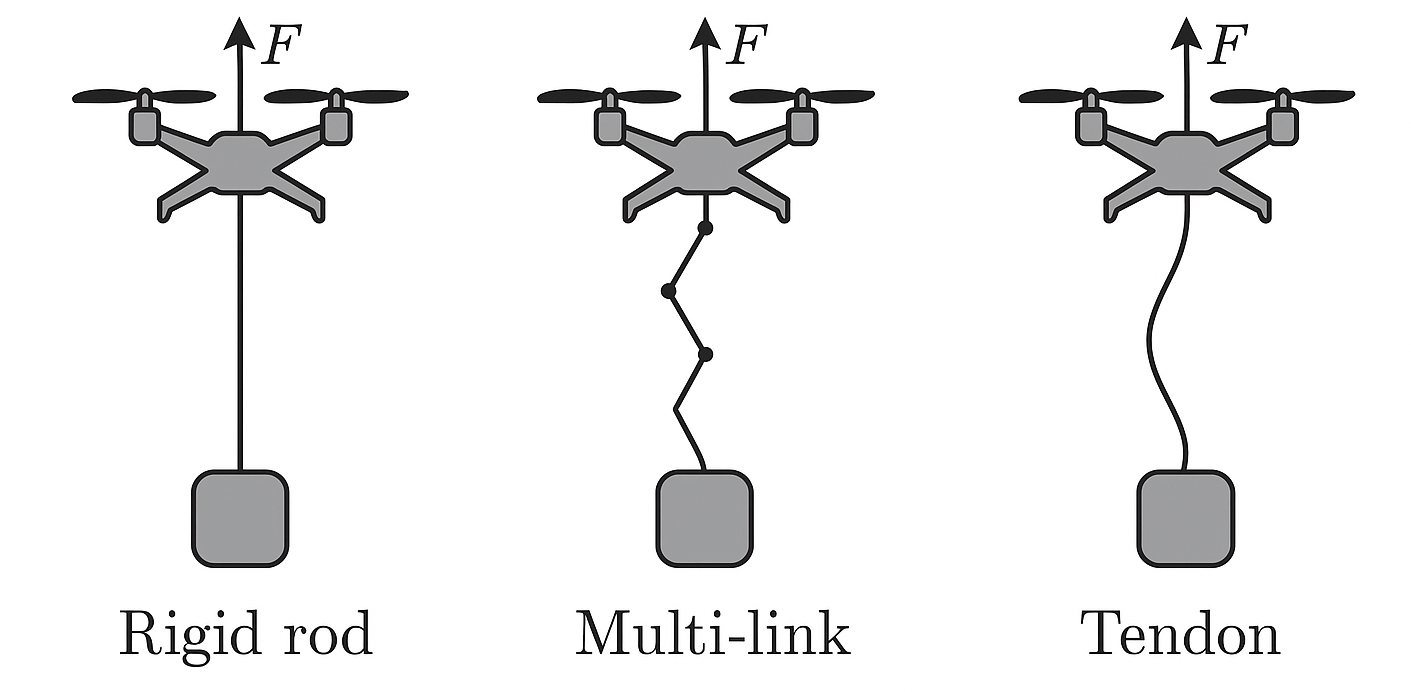
\includegraphics[width=0.6\textwidth]{cable_models.png}
  \caption{TODO Different approaches to modeling a cable-suspended payload. (a) A simple pendulum model with a rigid link and point-mass payload. (b) A multi-link pendulum model with \(N\) serial links. (c) A tendon approximation in MuJoCo}
  \label{fig:cable_models}
\end{figure}
Figure~\ref{fig:cable_models} illustrates three common cable‐suspended payload models.
When a quadrotor carries a cable-suspended payload, its state must be augmented to include cable and payload variables. A simple model treats the cable as a massless, inextensible rigid link of length \(\ell\), with a point-mass payload \(m_{L}\) at the end. The payload position \(\mathbf{p}_{L}\) relates to the quadrotor position \(\mathbf{p}_{Q}\) by
\[
\mathbf{p}_{L} \;=\; \mathbf{p}_{Q} \;-\; \ell\,\mathbf{q}, 
\quad
\|\mathbf{q}\| = 1,
\]
where \(\mathbf{q}\in S^{2}\) is the unit vector along the cable \cite{estevez_review_2024}. In this pendulum model, the augmented state is
\[
x_{\mathrm{aug}} 
= \bigl(\mathbf{p}_{Q},\,\mathbf{v}_{Q},\,\mathbf{R},\,\boldsymbol{\omega},\,\mathbf{q},\,\dot{\mathbf{q}}\bigr),
\]
with \(\mathbf{v}_{Q} = \dot{\mathbf{p}}_{Q}\) and \(\dot{\mathbf{q}}\) capturing payload swing \cite{Wahba2024}.

A more detailed multi-link pendulum model represents the cable as \(N\) serial, massless links of lengths \(\{\ell_{i}\}\), each with orientation \(\mathbf{q}_{i}\in S^{2}\). The payload position becomes
\[
\mathbf{p}_{L} 
= \mathbf{p}_{Q} \;-\; \sum_{i=1}^{N}\ell_{i}\,\mathbf{q}_{i},
\]
and the state is augmented by \(\{\mathbf{q}_{i},\,\dot{\mathbf{q}}_{i}\}_{i=1}^{N}\). This captures cable sag and higher-order swing modes but increases dimensionality from 8 (rigid link) to \(6 + 4N\), where 6 corresponds to \(\mathbf{p}_{Q},\,\mathbf{v}_{Q},\,\mathbf{R},\,\boldsymbol{\omega}\) \cite{goodarzi_dynamics_2015}.

In MuJoCo, cables are approximated as tendon elements. Tendons are massless, inelastic, high stiffness springs enforcing \(\|\mathbf{p}_{Q}-\mathbf{p}_{L}\| = \ell\) when taut. Tendons have no effect when they are slack. The augmented state reduces to
\[
x_{\mathrm{aug}} 
= \bigl(\mathbf{p}_{Q},\,\mathbf{v}_{Q},\,\mathbf{R},\,\boldsymbol{\omega},\,\mathbf{p}_{L},\,\mathbf{v}_{L}\bigr),
\]
where \(\mathbf{v}_{L} = \dot{\mathbf{p}}_{L}\). The tendon tension \(\mathbf{T}\) is applied only when the cable is taut and acts as \(-\mathbf{T}\) on the quadrotor and \(+\mathbf{T}\) on the payload in their dynamics.

For cooperative payload transport with \(M\) quadrotors, each quadrotor \(i\) has its own tendon to a common payload of mass \(m_{P}\). The payload dynamics are
\[
m_{P}\,\ddot{\mathbf{p}}_{P} 
= -m_{P}\,\mathbf{g} 
+ \sum_{i=1}^{M}\mathbf{T}_{i},
\]
and each quadrotor's translational dynamics include \(-\mathbf{T}_{i}\) alongside its collective thrust. The augmented state is
\[
x_{\mathrm{aug}} 
= \bigl(\{\mathbf{p}_{i},\,\mathbf{v}_{i},\,\mathbf{R}_{i},\,\boldsymbol{\omega}_{i}\}_{i=1}^{M},\,\mathbf{p}_{P},\,\mathbf{v}_{P}\bigr).
\]
This tendon approximation in MuJoCo captures essential characteristics of the hybrid dynamics, payload swing, tension variations, and multi-agent coordination, while remaining computationally efficient for simulation and control experiments.